\documentclass[letterpaper,11pt]{article}
\usepackage{graphicx}
\usepackage{listings}
\usepackage[super]{nth}
\usepackage[hyphens]{url}
\usepackage{hyperref}
\usepackage{amsmath}
\usepackage[makeroom]{cancel}
\usepackage[table]{xcolor}
\usepackage{comment}
\usepackage[space]{grffile}
\usepackage{csvsimple}
\usepackage{longtable}
\usepackage{adjustbox}


\newcommand*{\srcPath}{../src}%

\lstset{
	basicstyle=\footnotesize,
	breaklines=true,
}

\begin{document}

\begin{titlepage}

\begin{center}

\Huge{Assignment 10}

\Large{CS 532:  Introduction to Web Science}

\Large{Spring 2017}

\Large{Grant Atkins}

\Large Finished on \today

\end{center}

\end{titlepage}

\newpage


% =================================
% First question
% =================================
\section*{1}

\subsection*{Question}

\begin{verbatim}
1.  Using the data from A8:

- Consider each row in the blog-term matrix as a 
1000 dimension vector, corresponding to a blog.  

- From chapter 8, replace numpredict.euclidean() with 
cosine as the distance metric. In other words, you'll 
be computing the cosine between vectors of 1000 dimensions.  

- Use knnestimate() to compute the nearest neighbors for both:

http://f-measure.blogspot.com/
http://ws-dl.blogspot.com/

for k={1,2,5,10,20}.
\end{verbatim}

\clearpage
\subsection*{Answer}

To solve this question I used the blog data I previously received in assignment 8 \textbf{blogdata.txt} and the code provided by the Programming Collective Intelligence book \cite{collectiveIntell}. To calculate the cosine distance metric \textbf{numpredict.py} had to be modified to accompany this new function. The methods that changed in this file were the \textit{knnestimate} and \textit{getdistances} functions. In the \textit{getdistances} function I simply swapped out the euclidean function for cosine as shown in Listing \ref{lst:q1numpred}. In the \textit{knnestimate} function I removed the average value and instead return a list of sorted distances in descending order.

I then went filtered the F-measure and Web Science research group's blogs and create separate vectors with their values. These vectors were used for the cosine measurement against the vector with all blogs. This is shown in Listing \ref{lst:q1knncalc}.

\lstinputlisting[firstline=48,lastline=87,frame=single,caption={Python script with included cosine function and knnestimate changes},label=lst:q1numpred,captionpos=b,numbers=left,showspaces=false,showstringspaces=false,basicstyle=\footnotesize]{\srcPath/numpredict.py}

\lstinputlisting[frame=single,caption={Python script to find KNN values},label=lst:q1knncalc,captionpos=b,numbers=left,showspaces=false,showstringspaces=false,basicstyle=\footnotesize]{\srcPath/knn.py}

\clearpage
 \begin{figure}[h]
 \centering
 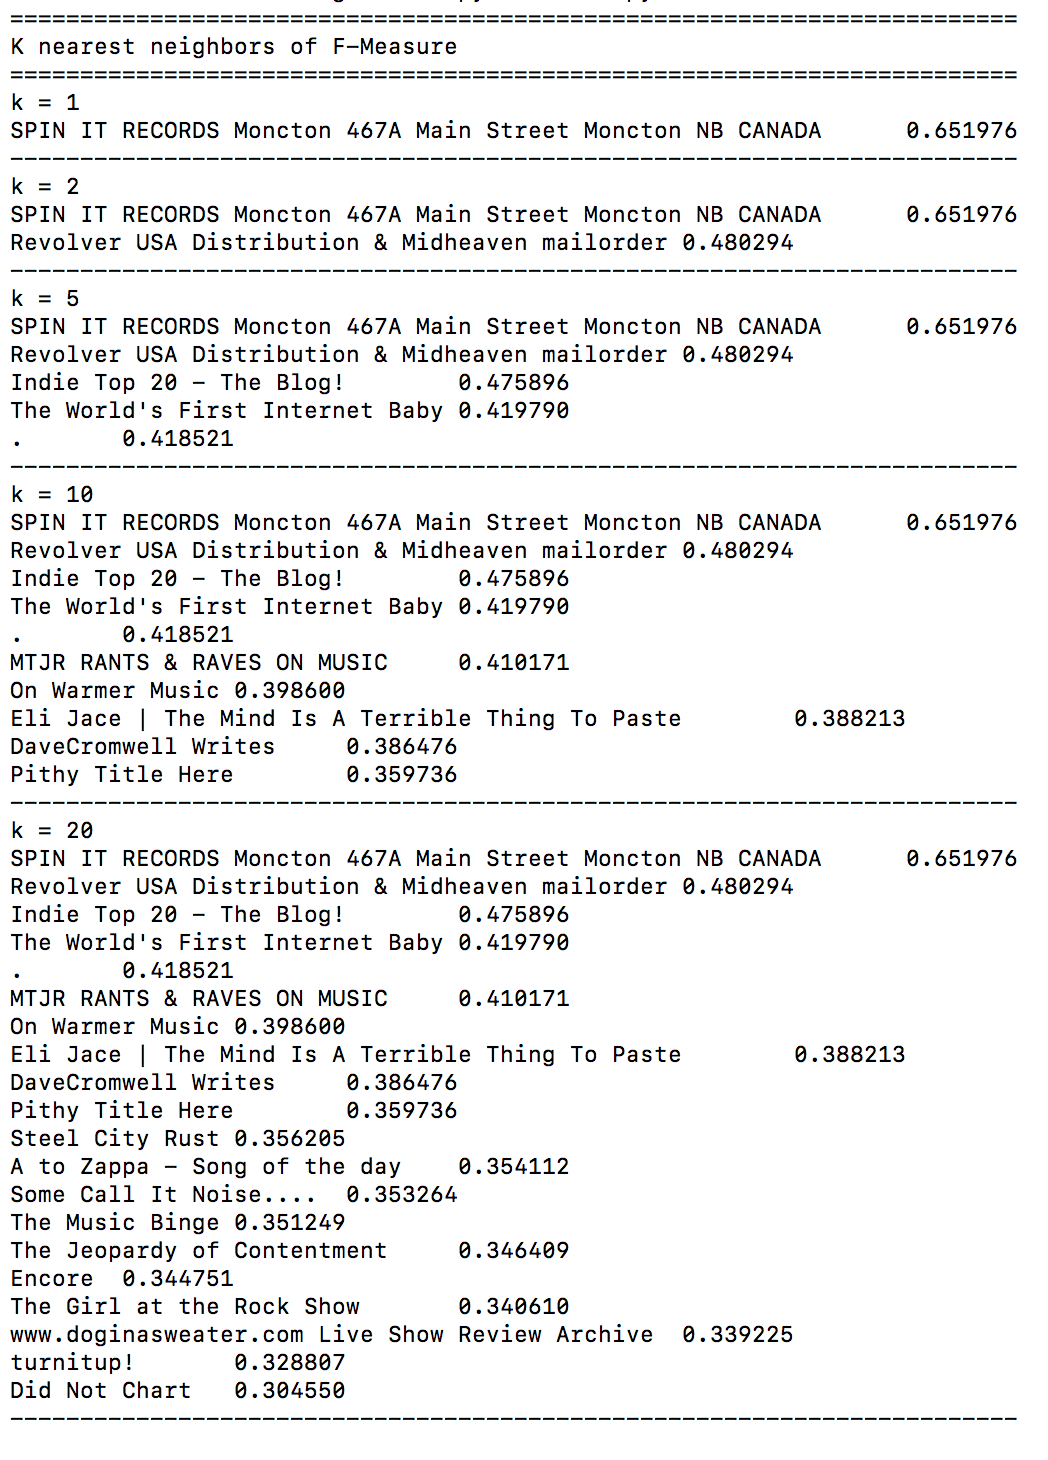
\includegraphics[scale=0.6]{fmeasureknn.png}
 \caption{F-Measure blog's KNNestimate output}
 \label{fig:q1knnout}
 \end{figure}

\clearpage
 \begin{figure}[h]
 \centering
 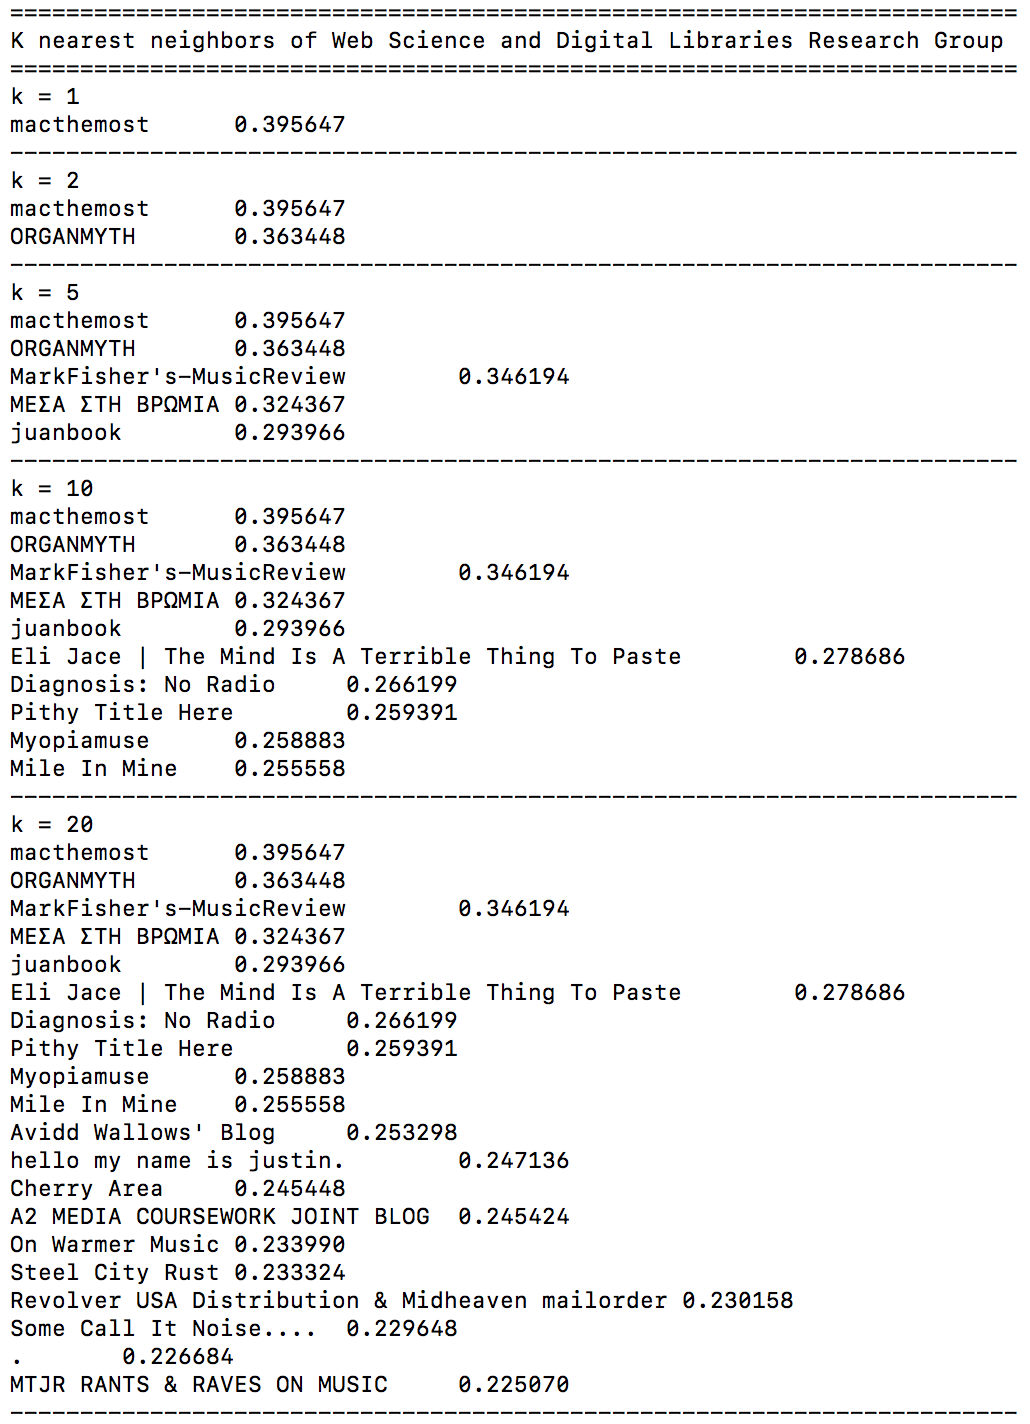
\includegraphics[scale=0.6]{webknn.png}
 \caption{Web Research group's KNNestimate output}
 \label{fig:q1webknn}
 \end{figure}


\clearpage

% =================================
% Second question
% =================================

\section*{2}

\subsection*{Question}

\begin{verbatim}
2.  Rerun A9, Q2 but this time using LIBSVM.  If you have 
n categories, you'll have to run it n times.  For example, 
if you're classifying music and have the categories:

metal, electronic, ambient, folk, hip-hop, pop

you'll have to classify things as:

metal / not-metal
electronic / not-electronic
ambient / not-ambient

etc.

Use the 1000 term vectors describing each blog as the features, and
your mannally assigned classifications as the true values.  Use
10-fold cross-validation (as per slide 46, which shows 4-fold
cross-validation) and report the percentage correct for 
each of your categories.
\end{verbatim}

\subsection*{Answer}

After reading many stackoverflow posts on LIBSVM, I decided to use the scikit-learn library to solve this question \cite{stack1}. I think this was a better option due to the ease of training and performing cross validation. When creating the blog matrix I combined the 100 selected feeds title and summary to create the new term matrix. Due to the short amount of text in each description it should be noted that my matrix creating program, \textbf{createMatrix.py} shown in Listing \ref{lst:q2createMatrix}, only created \textbf{898} terms instead of 1000. 

The actual SVM code for is shown in Listing \ref{lst:q2svm}. It first iterates through the newly created feed data matrix and matches my manual classification. A dictionary is created to hold all the values, it is then passed to the \textit{execSVM} function where it checks if the items have the category and performs SVM assigning values with 1 or -1 based if category was or was not the category assigned. Then finally performs cross validation folding up to 10 times.

\begin{table}[h]
\centering
\begin{adjustbox}{max width=\linewidth}
\begin{tabular}{ | l | l | l | l | l | l | l | l | l | l | l | l |}
\hline
\textbf{Category} & \textbf{Fold 1} & \textbf{Fold 2} & \textbf{Fold 3} & \textbf{Fold 4} & \textbf{Fold 5} & \textbf{Fold 6} & \textbf{Fold 7} & \textbf{Fold 8} & \textbf{Fold 9} & \textbf{Fold 10} & \textbf{Mean} \\
\hline
Android & 0.818182 & 0.800000 & 0.800000 & 0.800000 & 0.800000 & 0.800000 & 0.800000 & 0.800000 & 0.800000 & 0.888889 & 0.810707 \\ 
iOS & 0.818182 & 0.900000 & 0.600000 & 0.500000 & 0.900000 & 0.800000 & 0.800000 & 0.800000 & 0.900000 & 0.666667 & 0.768485 \\ 
Realm News & 0.727273 & 0.727273 & 0.727273 & 0.800000 & 0.800000 & 0.800000 & 0.800000 & 0.777778 & 0.777778 & 0.777778 & 0.771515 \\ 
React Native & 0.909091 & 0.909091 & 0.909091 & 0.909091 & 1.000000 & 1.000000 & 1.000000 & 1.000000 & 1.000000 & 1.000000 & 0.963636 \\ 
Nodejs & 0.909091 & 0.909091 & 0.909091 & 1.000000 & 1.000000 & 1.000000 & 1.000000 & 1.000000 & 1.000000 & 1.000000 & 0.972727 \\ 
Xamarin & 0.909091 & 0.909091 & 0.909091 & 0.909091 & 0.909091 & 1.000000 & 1.000000 & 1.000000 & 1.000000 & 1.000000 & 0.954545 \\ 
Databases & 0.909091 & 0.909091 & 0.909091 & 0.909091 & 0.909091 & 1.000000 & 1.000000 & 1.000000 & 1.000000 & 1.000000 & 0.954545 \\ 
\hline
\end{tabular}
\end{adjustbox}
\caption{SVM with 10-fold cross validation}
\label{table:q2cross}
\end{table}

\clearpage

\lstinputlisting[frame=single,caption={Python script to create term matrix from Realm RSS feed 100 items},label=lst:q2createMatrix,captionpos=b,numbers=left,showspaces=false,showstringspaces=false,basicstyle=\footnotesize]{\srcPath/createMatrix.py}

\lstinputlisting[frame=single,caption={Python script to perform cross validation with SVM classifier},label=lst:q2svm,captionpos=b,numbers=left,showspaces=false,showstringspaces=false,basicstyle=\footnotesize]{\srcPath/svm.py}

\clearpage

% =================================
% 3rd question
% =================================

\section*{3}

\subsection*{Question}

\begin{verbatim}
(3 points extra credit)

3. Re-download the 1000 TimeMaps from A2, Q2.  Create a graph where
the x-axis represents the 1000 TimeMaps.  If a TimeMap has "shrunk",
it will have a negative value below the x-axis corresponding to the
size difference between the two TimeMaps.  If it has stayed the
same, it will have a "0" value.  If it has grown, the value will be 
positive and correspond to the increase in size between the two
TimeMaps.

As always, upload all the TimeMap data.  If the A2 github has the 
original TimeMaps, then you can just point to where they are in 
the report.
\end{verbatim}

\subsection*{Answer}

\begin{center}
\Huge{NOT ATTEMPTED}
\end{center}

% \begin{figure}[h]
% \centering
% 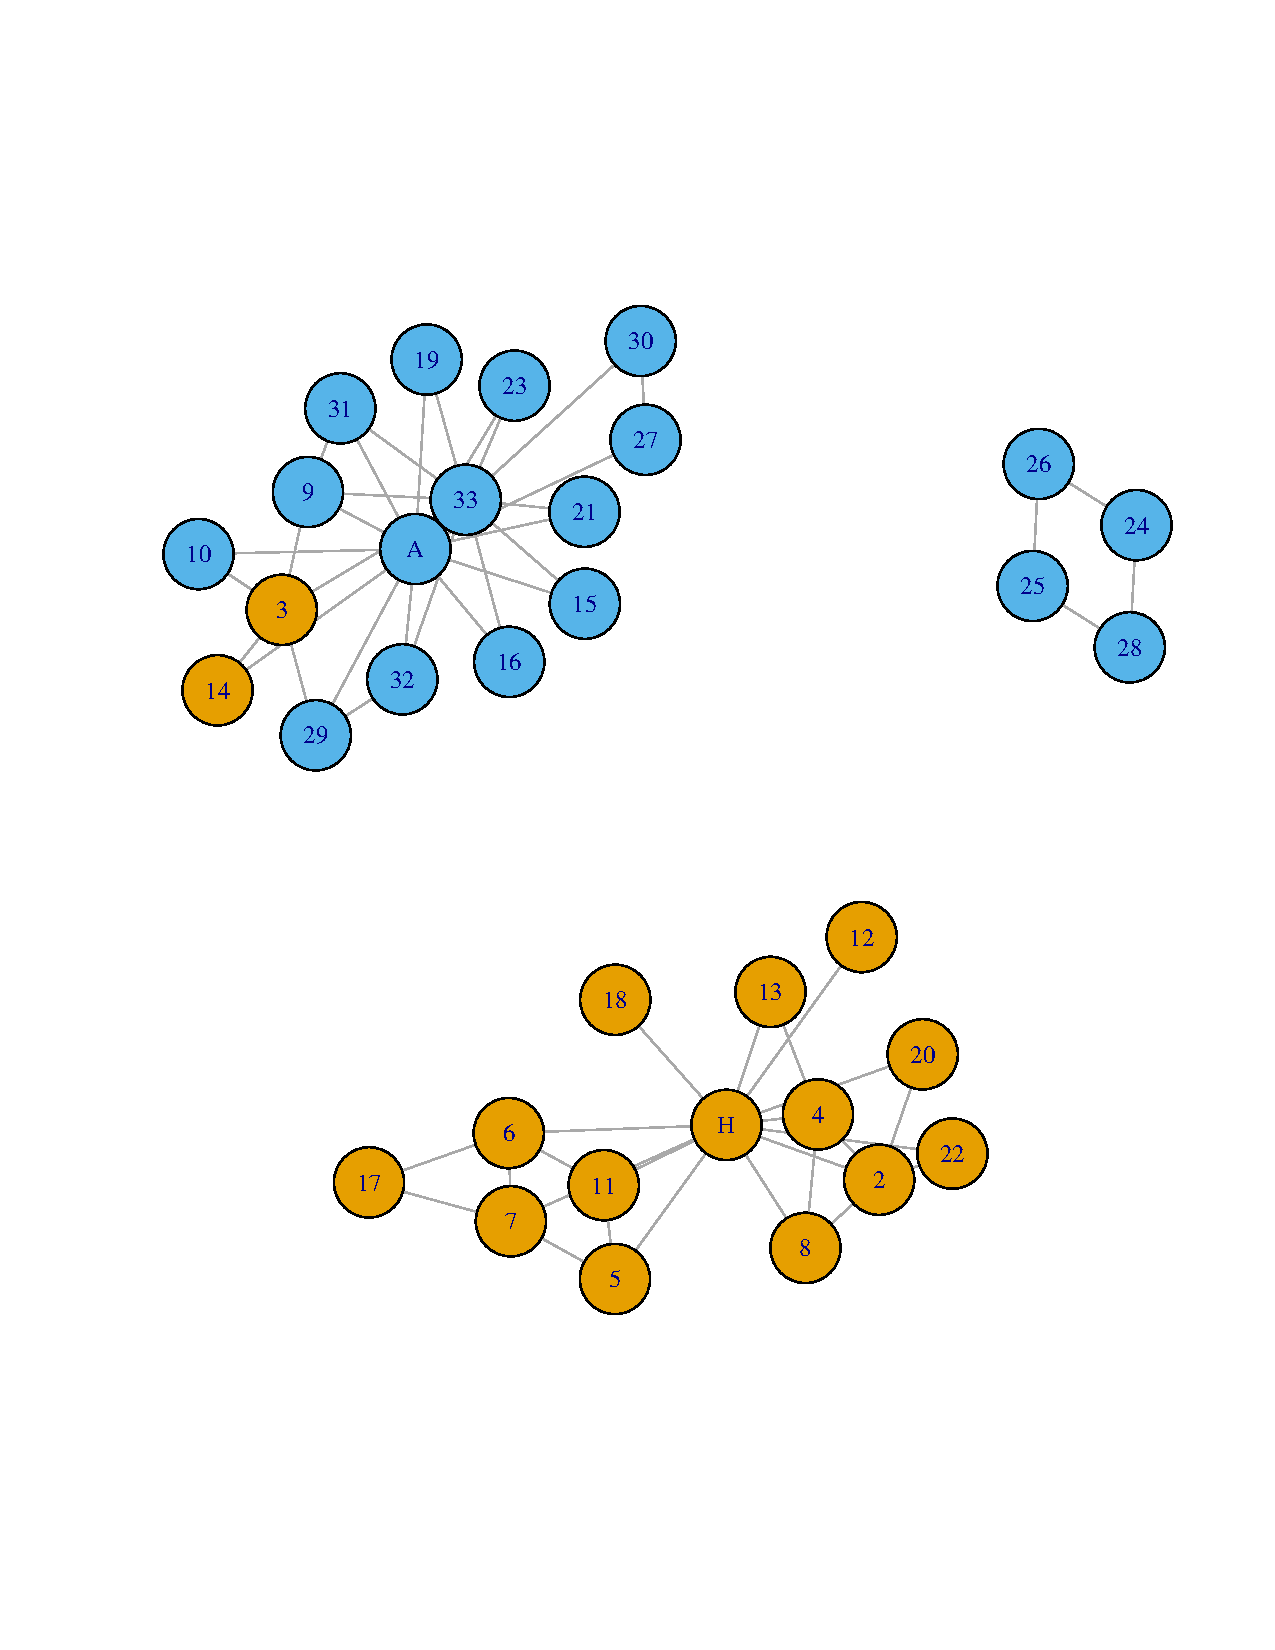
\includegraphics[scale=0.6]{predictedSplit3.pdf}
% \caption{Group split of 3 with Girvan-Newman algorithm from karateClub.R}
% \label{fig:split3}
% \end{figure}

\clearpage

% =================================
% 4th question
% =================================

\section*{4}

\subsection*{Question}

\begin{verbatim}
(3 points extra credit)

4.  Repeat A3, Q1.  Compare the resulting text from February to 
the text you have now.  Do all 1000 URIs still return a "200 OK" 
as their final response (i.e., at the end of possible redirects)?

Create two graphs similar to that described in Q3, except this 
time the y-axis corresponds to difference in bytes (and not difference
in TimeMap magnitudes).  For the first graph, use the difference
in the raw (unprocessed) results.  For the second graph, use the 
difference in the processed (as per A3, Q1) results.

Of the URIs that still terminate in a "200 OK" response, pick the
top 3 most changed (processed) pairs of pages and use the Unix
"diff" command to explore the differences in the version pairs.
\end{verbatim}

\subsection*{Answer}

Using the same code from A3 I downloaded the html files with the same URI list, which is also in my assignment 10 repository. The files to download the pages and process them are \textbf{download.sh} and textbf{processHtml.py} which aren't listed but are also in my repository. The only real file that required more work was done in two files, \textbf{fileSizeDiff.R} for histogram creation and \textbf{getFileSizes.py} which calculate the bytes for the old files processed and raw html files, as well as the new processed and raw html files.

I unfortunately did not have enough time to keep track of which URIs were actually still responding with a 200 response code. However I only included URIs in the charts below that still returned content and matched the final URI of the previous one found in assignment 3. The bar charts below indicate the old file size in bytes minus the new file size in bytes.

 \begin{figure}[h]
 \centering
 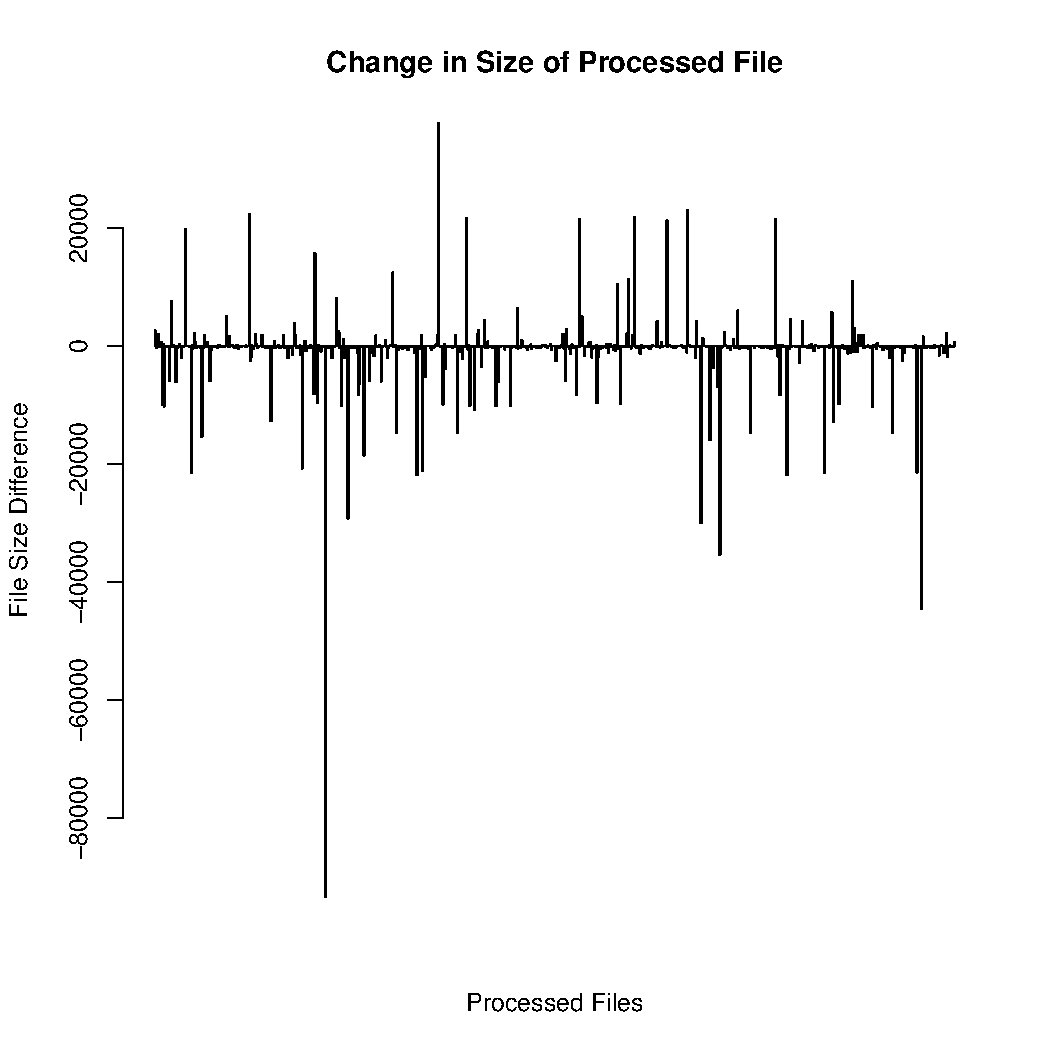
\includegraphics[scale=0.8]{ProcessedHistogram.pdf}
 \caption{Barplot of Processed files in bytes, the new value is old byte size minus new byte size}
 \label{fig:q3split3}
 \end{figure}
 
  \begin{figure}[h]
 \centering
 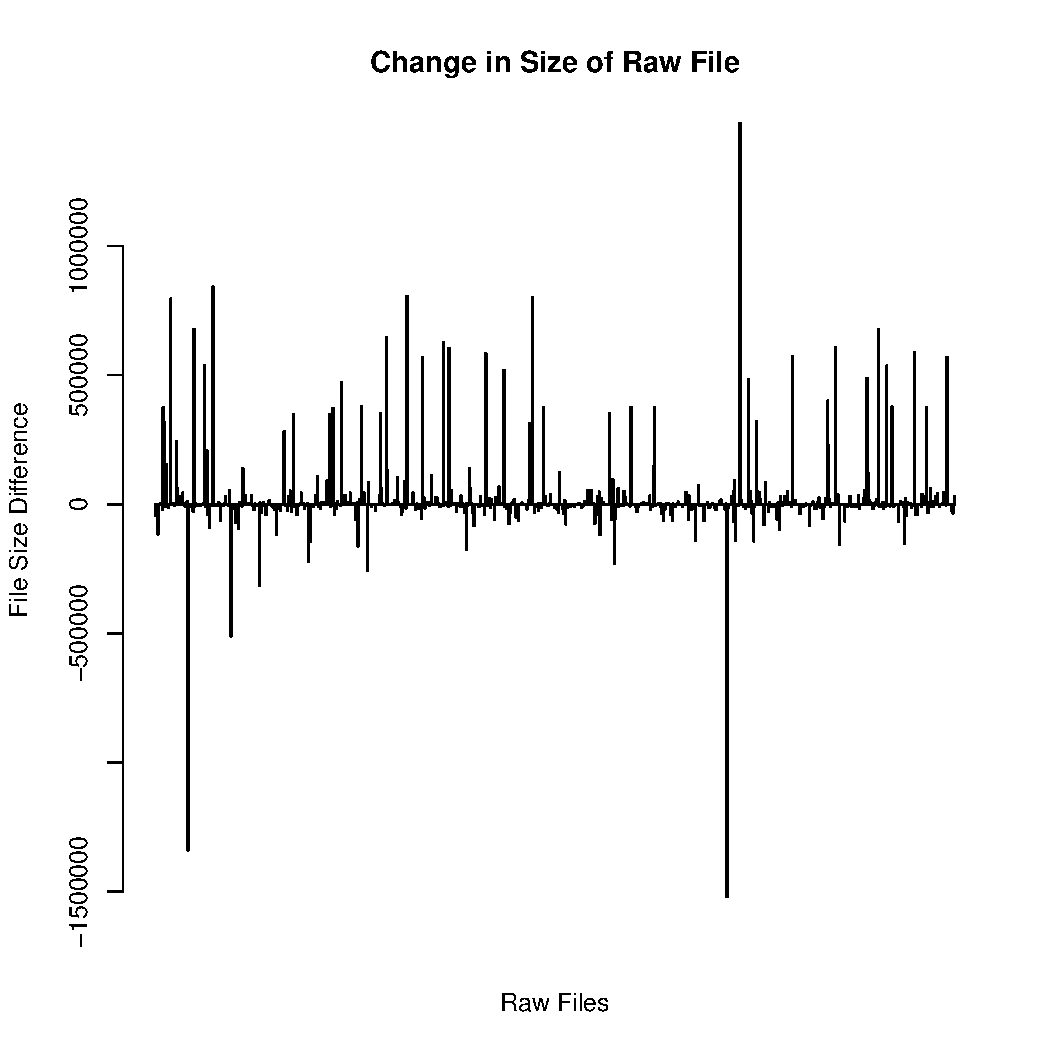
\includegraphics[scale=0.8]{RawHistogram.pdf}
 \caption{Barplot of Raw files in bytes, the new value is old byte size minus new byte size}
 \label{fig:q3split4}
 \end{figure}

\clearpage


\clearpage


% =================================
% Bibliography
% =================================

\begin{thebibliography}{9}
\bibitem{github}
Atkins, Grant. ``CS532 Assignment 10 Repository'' Github. N.p., 23 March 2017. Web. 23 March 2017.\url{https://github.com/grantat/cs532-s17/tree/master/assignments/A10}.
\bibitem{collectiveIntell}
Segaran, Toby. ``Programming Collective Intelligence''. O' Reilly, 2007. Web. 6 April 2017. \url{http://shop.oreilly.com/product/9780596529321.do}.
\bibitem{stack1}
``How to setup LIBSVM for Python''. n.p., n.d. Web. 1 May 2017. \url{http://stackoverflow.com/questions/15755130/how-to-setup-libsvm-for-python}
\end{thebibliography}

\end{document}